\documentclass[twoside,11pt]{article}

% Any additional packages needed should be included after jmlr2e.
% Note that jmlr2e.sty includes epsfig, amssymb, natbib and graphicx,
% and defines many common macros, such as 'proof' and 'example'.
%
% It also sets the bibliographystyle to plainnat; for more information on
% natbib citation styles, see the natbib documentation, a copy of which
% is archived at http://www.jmlr.org/format/natbib.pdf

\usepackage{jmlr2e}

\usepackage[acronym]{glossaries} %Used for the acronyms
\usepackage{mathtools} %tools for mathematical writing
\usepackage{caption}
\usepackage{subfig}
\usepackage{float}
\usepackage{color}
\usepackage{adjustbox}
\usepackage{comment}
\usepackage{hyperref} % For hyperlinks in the PDF
\usepackage{algorithm}% http://ctan.org/pkg/algorithms
\usepackage{algpseudocode}% http://ctan.org/pkg/algorithmicx
\usepackage[acronym]{glossaries} %Used for the acronyms
\usepackage[titletoc]{appendix}

% Definitions of handy macros can go here

\newcommand{\dataset}{{\cal D}}
\newcommand{\fracpartial}[2]{\frac{\partial #1}{\partial  #2}}

% Heading arguments are {volume}{year}{pages}{date submitted}{date published}{paper id}{author-full-names}

\jmlrheading{18}{2018}{1-48}{07/18}{10/00}{dlaredo00a}{Laredo, Chen, Sun and Sch\"{u}tze}

% Short headings should be running head and authors last names

\ShortHeadings{Evolutionary Computation Framework for Remaining Useful Life Estimation}{Laredo, Chen,  Sun and Sch\"{u}tze}
\firstpageno{1}

\begin{document}

\title{A Neural Network-Evolutionary Computation Framework for Remaining Useful Life Estimation}

%Term definitions
\newacronym{rul}{RUL}{Remaining Useful Life}
\newacronym{mlp}{MLP}{Multi-layer Perceptron}
\newacronym{cmaps}{C-MAPSS}{Commercial Modular Aero Propulsion System Simulator}
\newacronym{ann}{ANN}{Arificial Neural Networks}
\newacronym{cbm}{CBM}{Condition Based Maintenance}
\newacronym{pmh}{PMH}{Prognostics and Health Management}
\newacronym{ml}{ML}{Machine Learning}



%Remove after the paper is complete.
\newacronym{moo}{MOO}{Multi-objective Optimization}
\newacronym{mop}{MOP}{Multi-objective Optimization Problem}
\newacronym{mmop}{MMOP}{Mixed-Integer Multi-objective Optimization Problem}
\newacronym{eds}{EDS}{Enhanced Directed Search}
\newacronym{dzz}{DZZ}{Direct Zig Zag}
\newacronym{nsga2}{NSGA-II}{Non-Sorted Genetic Algorithm II}
\newacronym{sop}{SOP}{Single-objective Optimization Problem}
\newacronym{pc}{PC}{Predictor-Corrector}
\newacronym{moea}{MOEA}{Multi-objective Optimization Evolutionary Algorithm}
\newacronym{ea}{EA}{Evolutionary Algorithm}
\newacronym{ds}{DS}{Directed Search}
\newacronym{kkt}{KKT}{Karush-Kuhn-Tucker}
\newacronym{bop}{BOP}{Bi-objective Optimization Problem}
\newacronym{gd}{GD}{Generational Distance}
\newacronym{igd}{IGD}{Inverted Generational Distance}
\newacronym{gsa}{GSA}{Gradient Subspace Approximation}
\newacronym{ift}{IFT}{Implicit Function Theorem}
\newacronym{fps}{FPS}{First Pareto Solution}
\newacronym{moead}{MOEA-D}{Multi-objective Optimization Evolutionary Algorithm based on Decomposition}
\newacronym{pf}{PF}{Pareto Front}
\newacronym{nbi}{NBI}{Normal Boundary Intersection}
\newacronym{pso}{PSO}{Particle Swarm Optimization}
 %Insert acronym list

%Used to not expand the first acronym
\glsunsetall

\author{\name David Laredo \email dlaredorazo@ucmerced.edu \\
			 \name Zhaoyin Chen \email zchen@ucmerced.edu \\
			 \name Jian-Qiao Sun \email jsun3@ucmerced.edu \\
       \addr Department of Mechanical Engineering\\
       University of California\\
       Merced, Ca 95340-5200, USA
       \AND
       \name Oliver Sch\"{u}tze \email schuetze@cs.cinvestav.mx \\
       \addr Department of Computer Science\\
       CINVESTAV\\
       Mexico City, Av. Instituto Politecnico Nacional 07360-1776, Mexico}

\editor{Kevin Murphy and Bernhard Sch{\"o}lkopf}

\maketitle

\begin{abstract}%   <- trailing '%' for backward compatibility of .sty file
This paper presents a data-driven framework for estimating the remaining useful life (\gls{rul}) of mechanical systems. Two major components make up the framework: a multi-layer perceptron as base regressor and an evolutionary computation algorithm for the tuning of data-related parameters. On the data side, the framework makes use of a strided time window along with a piecewise linear model to estimate the \gls{rul} label for each time window within the training sets. Tuning the data-related parameters using the optimization framework here presented allows for the use of simple regressor models, e.g. neural networks with few hidden layers and few neurons at each layer, which can in turn be deployed in environments with very limited resources such as embedded systems. The proposed method is evaluated on the publicly available \gls{cmaps} dataset. The accuracy of the proposed method is compared against other state-of-the art methods available in the literature and it is shown to perform better while making use of a simpler, compact model.
\end{abstract}

\begin{keywords}
  Artificial Neural Networks, Moving Time Window, \gls{rul} Estimation, Prognostics, Evolutionary Algorithms
\end{keywords}

%----------------------------------------------------------------------------------------
%	ARTICLE CONTENTS
%----------------------------------------------------------------------------------------

\section{Introduction}
\label{sec:rul_intro}

Traditionally, maintenance of mechanical systems has been carried out based on scheduling strategies, nevertheless such strategies are often costly and less capable of meeting the increasing demand of efficiency and reliability \cite{Gebraeel2005, Zaidan2013}. Condition Based Maintenance (\gls{cbm}) also known as intelligent Prognostics and Health Management (\gls{pmh}) allows for maintenance based on the current health of the system, thus cutting costs and increasing the reliability of the system \cite{Zhao2017}. To avoid confusion, here we define prognostics as the estimation of remaining useful component life. The Remaining Useful Life (\gls{rul}) of a system can be estimated based on history trajectory data, this approach which we refer here as data-driven can help improve maintenance schedules to avoid engineering failures and save costs \cite{Lee2014}.

The existing \gls{pmh} methods can be grouped into three different categories: model-based \cite{Yu2001} , data-driven \cite{Liu2009, Mosallam2013} and hybrid approaches \cite{Pecht2010, Liu2012}.

Model-based approaches attempt to incorporate physical models of the system into the estimation of the \gls{rul}. If the system degradation is modeled  precisely, model-based approaches usually exhibit better performance than data-driven approaches \cite{Qian2017}, nevertheless this comes at the expense of having extensive a prior knowledge of the underlying system and having a fine-grained model of such system (which usually involve expensive computations). On the other hand data-driven approaches tend to use pattern recognition to detect changes in system states. Data-driven approaches are appropriate when the understanding of first principles of system operation is not comprehensive or when the system is sufficiently complex (i.e. jet engines, car engines, complex machinery) such that developing an accurate model is prohibitively expensive. Common disadvantages for the data-driven approaches are that they usually exhibit wider confidence intervals than model-based approaches and that a fair amount of data is required for training. Many data-driven algorithms have been proposed and good prognostics results have been achieved, among the most popular algorithms we can find Artificial Neural Networks (\gls{ann}) \cite{Gebraeel2004}, Support Vector Machine (\gls{svm}) \cite{Benkedjouh2013}, Markov Hidden Chains (\gls{mhc}) \cite{Dong2007}.

Over the past few years, data-driven approaches have gained more attention in the \gls{pmh} community. A number of machine learning techniques, especially neural networks have been successfully applied to the estimate \gls{rul} of diverse mechanical systems. \glspl{ann} have demonstrated good performance when applied for modeling highly nonlinear, complex, multi-dimensional system without any prior expertise on the system's physical behavior \cite{Li2018}. While the confidence limits for the \gls{rul} predictions can not be naturally provided \cite{Sikorska2011}, the neural network approaches are promising on prognostic problems.

Neural Networks for estimating the \gls{rul} of jet engines has been previously explored in \cite{Lim2016} where the authors propose a Multi-layer Perceptron \gls{mlp} coupled with a Feature Extraction (\gls{fe}) method and a time window for the generation of the features for the \gls{mlp}. In the publication the authors demonstrate that a moving window combined with a suitable feature extractior can improve the \gls{rul} prediction reported by other similar methods in the literature. In \cite{Li2018} the authors explore an even newer \gls{ann} architecture, the so-called Convolutional Neural Networks \glspl{cnn}, where they demonstrate that by using a \gls{cnn} without any pooling layers coupled with a time-window the predicted \gls{rul} is further improved.

In this paper we propose a novel framework for estimating the \gls{rul} of complex mechanical systems. The framework consists of a Multi-layer Perceptron (\gls{mlp}) to estimate the \gls{rul} of the system at hand, coupled with an evolutionary algorithm for the fine tuning of data-related parameters, i.e. parameters that define the shape and quality of the features used by the \gls{mlp}. The publicly available NASA \gls{cmaps} dataset \cite{CMAPS2008} is used to assess the efficiency and reliability of the proposed framework. This approach allows for even simple and small \glspl{mlp}, thus being suitable for computationally restricted environments, to obtain better results than those reported in the current literature while using less computing power.

The remainder of this paper is organized as follows: The \gls{cmaps} dataset is presented in Section \ref{sec:rul_dataset}, then the framework and all of its components are thoroughly reviewed in Section \ref{sec:method}. The method is evaluated using the \gls{cmaps} dataset in Section \ref{sec:rul_eval}, a comparison with the state-of-the-art is also provided. Finally, our conclusions are presented in Section \ref{sec:conclusions}.
\section{NASA C-MAPSS Dataset}
\label{sec:rul_dataset}

The NASA \gls{cmaps} dataset \cite{CMAPS2008} is used to evaluate the proposed method. The \gls{cmaps} dataset contains simulated data produced using a model based simulation program (Commercial Modular Aero-Propulsion System Simulation) developed by NASA. The dataset is further divided into 4 subsets composed of multi-variate temporal data obtained from 21 sensors.

For each of the 4 subsets a training and a test set is provided. The training sets include run-to-failure sensor records of multiple aero-engines collected under different operational conditions and fault modes as described in Table \ref{table:cmapss}

The data is arranged in an $n\times26$ matrix where $n$ corresponds to the number of data points in each subset. The first two variables represent the engine and cycle numbers respectively. The following three variables are operational settings which correspond to the operating conditions in Table \ref{table:cmapss} and have a substantial effect on engine performance. The remaining variables represent the 21 sensor readings that model the engine degradation throughout time.

\begin{table}[!htb]
\centering
\begin{tabular}{l | l l l l}
	\hline
	 & \multicolumn{4}{c}{C-MAPSS}\\  
	 Dataset & FD001 & FD002 & FD003 & FD004\\
  	\hline
  	Train Trajectories & 100 & 260 & 100 & 248\\
  	Test Trajectories & 100 & 259 & 100 & 248\\
  	Operating Conditions & 1 & 6 & 1 & 6\\
  	Fault Modes & 1 & 1 & 2 & 2\\
  	\hline
\end{tabular}
\caption{C-MAPSS Dataset details}
\label{table:cmapss}
\end{table}

Each trajectory within the train and test trajectories is assumed to represent the life-cycle of an engine. Each engine is simulated with different initial health conditions (no faults). For each trajectory of an engine the last data entry corresponds to the moment the engine is declared faulty. On the other hand the trajectories within the test sets terminate at some point prior to failure  and the aim is to predict the Remaining Useful Life (\gls{rul}) of each engine in the test set. The actual \gls{rul} value of each test trajectories were also included in the dataset for verification purposes. Further discussion of the dataset and details on how the data is generated are given in \cite{Saxena2008}.

\subsection{Performance evaluation}
\label{sec:rul_metrics}

The evaluate the performance of the proposed approach on the \gls{cmaps} dataset we make use of two scoring indicators, namely the Root Mean Squared Error (\gls{rmse}) and a score function proposed in \cite{Saxena2008} which we refer in this work as \gls{rul} Health Score (\gls{rhs}). 

\begin{equation}
RMSE = \sqrt{ \frac{1}{N} \sum_{i=1}^{N}{d_i^2}}
\end{equation}

\begin{align}
s &= \sum_{i=1}^{N}{s_i}\\
s_i &= \begin{cases} 
      e^{-\frac{d_i}{13}} - 1 & d_i < 0, \\
      e^{-\frac{d_i}{10}} - 1 & d_i \geq 0
\end{cases}
\end{align}

where $s$ denotes the score and $N$ is the total number of testing data samples. $d_i = RUL_i^p - RUL_i$, that is the error between the estimated \gls{rul} value and the actual \gls{rul} value for the \textbf{i-th} testing sample. The (\gls{rhs}) function penalizes late predictions more than early predictions since usually late predictions lead to more severe consequences in fields such as aerospace.


%\section{Performance evaluation}
\label{sec:rul_metrics}

The evaluate the performance of the proposed approach we make use of two scoring indicators, namely the Root Mean Squared Error (\gls{rmse}) and a score function proposed in \cite{Saxena2008} which we refer in this work as \gls{rul} Health Score (\gls{rhs}). 

\begin{equation}
RMSE = \sqrt{ \frac{1}{N} \sum_{i=1}^{N}{d_i^2}}
\end{equation}

\begin{align}
s &= \sum_{i=1}^{N}{s_i}\\
s_i &= \begin{cases} 
      e^{-\frac{d_i}{13}} - 1 & d_i < 0, \\
      e^{-\frac{d_i}{10}} - 1 & d_i \geq 0
\end{cases}
\end{align}

where $s$ denotes the score and $N$ is the total number of testing data samples. $d_i = RUL_i^p - RUL_i$, that is the error between the estimated \gls{rul} value and the actual \gls{rul} value for the \textbf{i-th} testing sample. The (\gls{rhs}) function penalizes late predictions more than early predictions since usually late predictions lead to more severe consequences in fields such as aerospace.


%\section{Artificial Neural Networks}
\label{sec:rul_ann}

Although Artificial Neural Networks (\glspl{ann}) are widely know nowadays in this section we will briefly introduce the basic concepts behind them to provide the reader a better understanding of the tools used in this work. We will follow the notation and conventions used in \cite{Engelbrecht2007}

Artificial Neural Networks (\glspl{ann}) are systems vaguely inspired by the biological Neural Networks in the brain. Neurons are the building blocks of any type of \gls{ann}. The Artificial Neuron \gls{an}, or neuron, implements a nonlinear mapping from $\mathbb{R}^{n}$ to $\left[a,b\right]$ where $n$ is the number of inputs the \gls{an} receives and $a$ and $b$ depend on the chosen activation function. Usual combinations for $a$ and $b$ are $\left[0,1\right]$ or $\left[-1,1\right]$

\begin{equation}
f_{AN} : \mathbb{R}^n \rightarrow \left[a,b\right]
\label{eq:an_def}
\end{equation}

An \gls{an} receives a vector of $n$ input signals, $\mathbf{z} = (z_1, z_2, \cdots , z_n)$, either from the environment or from other \glspl{an}. The \gls{an} computes the net input signal, and uses an activation function $f_{AN}$ to compute the output signal, $o$, given the net input. The strength of the output signal is further influenced by a bias value $\theta$. Figure \ref{fig:an_1} presents an illustration of an \gls{an}.

\begin{figure}[h]
    \centering
    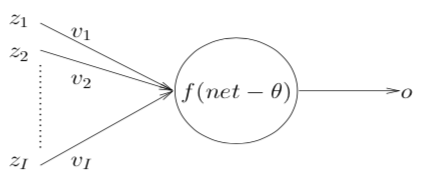
\includegraphics[width = 50mm, height = 25mm]{img/artificial_neuron.png}
    \caption{An Artificial Neuron} 
    \label{fig:an_1}
\end{figure}

The net input signal to an \gls{an} is usually computed as the weighted sum of all input signals.

\begin{equation}
net = \sum_{i=1}^n z_i v_i
\label{eq:an_net}
\end{equation}

The function $f_{AN}$ receives the net input signal and bias, and determines the output of the neuron. This function is referred as the \textit{activation function}. Different types of activation functions can be used \cite{Engelbrecht2007}, among the most popular ones we find the sigmoid function, tanh function and the newer Rectified Linear Unit (\gls{relu}) function. The values of the weights $\nu_i$ and the bias $\theta$ are adjusted through an optimization process. In supervised learning the \gls{an} is provided with a dataset consisting of input vectors and a target (desired output) associated with each input vector. This data is referred as training set. The aim is then to adjust the weight values and bias such that the error between the real output, $o = f(net - \theta)$, of the neuron and the target output, $t$, is minimized.

\begin{figure}[h]
    \centering
    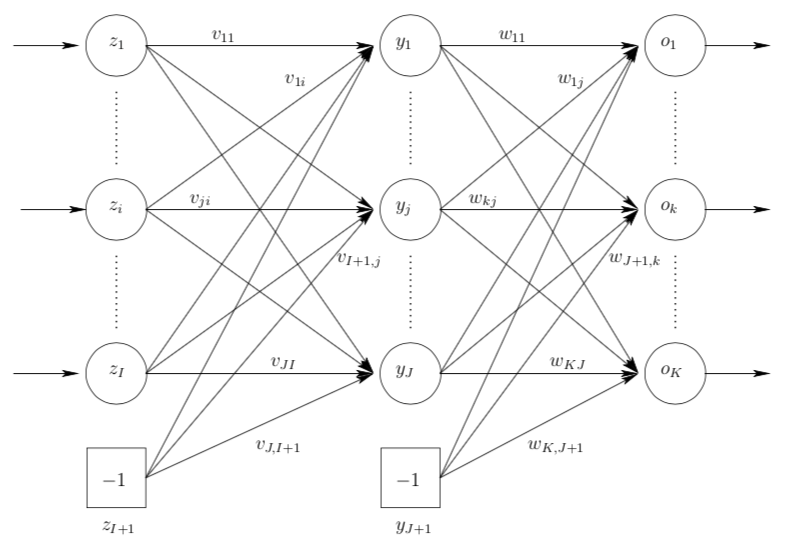
\includegraphics[width = 100mm, height = 50mm]{img/artificial_neural_network.png}
    \caption{A Multi-layer Perceptron} 
    \label{fig:ann_1}
\end{figure}

By stacking several neurons together to form an output vector $\mathbf{o} = (o_1, o_2, \cdots \o_m)$ (a layer) and then using $\mathbf{o}$ as the input to another set of neurons and so on we can form the so-called Multi-layer Perceptron (\gls{mlp}). The layers of the \gls{mlp} in between the input and output layers are called hidden layers. Figure \ graphically depicts a \gls{mlp} with one hidden layer. The process of adapting the weight matrices at each layer is called training of the Neural Network and is described in detail in \cite{Engelbrecht2007}.
\section{Estimating Remaining Useful Life using Multi-Layer Perceptron as Regressor}
\label{sec:method}

In this section the proposed \gls{ann}-based method for prognostics is presented. Our method uses a Multi-Layer Perceptron (\gls{mlp}) as the main regressor for estimating the \gls{rul} of the engines at each subset of the \gls{cmaps} dataset. For the training sets, the feature vectors are generated by using a strided time window while the labels vector is generated using a constant \gls{rul} for the early cycles of the simulation and then linearly decreasing the number of remaining cycles, this is the so called piecewise linear degradation model \cite{Ramasso2014}. For the test set, a time window is taken from the last sensor readings of the engine and used to predict the \gls{rul} of the engine.

The window size $n_w$, window stride $n_s$ and early \gls{rul} $R_e$ data related parameters have a considerable impact in the quality of the predictions made by the regressor. Hand picking the best parameters for our application is time consuming, furthermore, a grid search approach as the ones used for hyperparameter tuning in Neural Networks is computationally expensive given the search space inherent to the aforementioned parameters. In this paper we propose the use of an evolutionary algorithm, i.e. Differential Evolution (\gls{de}) \cite{Storn1997}, to fine tune the parameters. The optimization framework here proposed allows for the use of a simple Neural Network architecture while attaining better results in terms of the quality of the predictions made than the ones in the current literature.

\subsection{The Neural Network Architecture}

For this study we propose to use a rather simple \gls{mlp} architecture. All the implementations were used in python using the Keras/Tensorflow environment. The structure of the Network remained consisted for all the four datasets.

The choice of the network architecture was made using an iterative process; comparing 4 different architectures, running each $10$ times for $100$ epochs and using a mini-batch size of $512$. Two objectives were pursued; that the size of the architecture was small enough, e.g. in terms of layers and neurons within each layer and that the performance indicators were better than the ones presented in the literature so far. The process for choosing the network architecture can be described as follows: First, fix the window size $n_w$, the window stride $n_s$ and the early RUL $R_e$. An initial setup of two layers with $250$ and $50$ neurons each was chosen, the number of neurons at each layer was then reduced by roughly a factor of 2 and tested using a cross-validation set from subset 1 of \gls{cmaps}. When the performance of the network started to degrade the process was stopped. Table  \ref{table:tested_architectures_100} summarizes the results for each tested architecture, Table \ref{table:proposed_nn} presents the architecture chosen for the remainder of this work yielded the best results and hence was the chosen for the rest of the experiments. Details for the other 3 tested architectures are presented in Section ...

\begin{table}[!htb]
\centering
\begin{tabular}{l r r | r r | r r | r r}
	\hline	
	& \multicolumn{2}{c}{Min.} & \multicolumn{2}{c}{Max.}  & \multicolumn{2}{c}{Avg.}  & \multicolumn{2}{c}{STD} \\
	Tested Architecture & RMSE & RHS & RMSE & RHS & RMSE & RHS & RMSE & RHS\\
  	\hline
  	Architecture 1 & 10.85 & 151.65 & 12.23 & 277.67 & 11.66 & 226.94 & 0.45 & 41.58\\
  	Architecture 2 & 11.12 & 186.22 & 13.98 & 365.92 & 12.68 & 280.41 & 1.03 & 64.07\\
  	Architecture 3 & 11.58 & 179.15 & 12.72 & 266.55 & 12.04 & 215.09 & 0.35 & 28.39\\
  	Architecture 4 & 12.52 & 262.77 & 14.25 & 368.35 & 13.58 & 325.41 & 0.53 & 34.13\\
  	\hline
\end{tabular}
\caption{Results for different architectures for subset 1, 100 epochs}
\label{table:tested_architectures_100}
\end{table}

\begin{table}[!htb]
\centering
\begin{tabular}{l l l l}
	\hline
	Layer & Shape & Activation & Additional Information\\
  	\hline
  	Fully connected & 30 & ReLU & Dropout(0.6)\\
  	Fully connected & 10 & ReLU & Dropout(0.2)\\
  	Fully connected & 1 & Linear & \\
  	\hline
\end{tabular}
\caption{Proposed Neural Network architecture}
\label{table:proposed_nn}
\end{table}

\subsection{Shaping the data}

This section covers the data preprocessing applied to the raw sensor readings in each of the datasets. Even-though the original datasets contains $21$ different sensor readings some of the sensor do not present much variance and are therefore discarded. Therefore only $14$ sensor readings out of the $21$ are considered for this study, their indices are $\left\lbrace 2, 3, 4, 7, 8, 9, 11, 12, 13, 14, 15, 17, 20, 21 \right\rbrace$. The raw measurements are then used to create the strided time windows with window size $n_w$ and window stride $n_s$, for the labels $R_e$ is used at the early stages and then the \gls{rul} is linearly decreased. Finally, the data is normalized to be within the range $\left[ -1,1 \right]$ using the min-max normalization.

\begin{equation}
x^{i,j}_{norm} = 2 \frac{x^{i,j} - x^{j}_{min}}{x^{j}_{max} - x^{j}_{min}} - 1
\label{eq:min_max_norm}
\end{equation}

where $x_{i,j}$ denotes the original $i$-th data point of the $j$-th sensor and $x^{i,j_norm}$ is the normalized value of $x^{i,j}$.  $x^{j}_{max}$ and $x^{j}_{min}$ denote the maximum and minimum values of the original measurement data from the $j$-th sensor, respectively. 

\subsubsection{Time Window Processing}

In multivariate time-series based problems such as \gls{rul}, more information can be generally obtained from the temporal sequence of data as compared with the multivariate data point at a single time stamp. Let $n_w$ denote the size of the time window, for a time window with a stride $n_s = 1$, all the past sensor values within the time window are collected and put together to form a feature vector $\mathbf{x}$. This approach has successfully been tested in \cite{Li2018, Lim2016} where they propose the use of a moving window with values raging from 20 to 30. In this paper we propose not only the use of a moving time window, but also a \textit{strided} time window that updates $n_s$ elements at the time instead of $1$. 

The use of a \textit{strided time window} allows for the regressor to take advantage not only of the previous information available, but also to control the ratio at which the algorithm is fed with new information. With the usual time window approach only one point is updated for every new time window, on the contrary, the strided time window allows for updating $n_s$ points at the time, allowing for the algorithm to catch newer information with fewer iterations, furthermore, the information contained in the strided time window is likely more rich than the one contained in a time window with stride of $1$.

\subsubsection{Piecewise linear degradation model}

Different from common regression problems, the desired output value of the input data is difficult to determine for a \gls{rul} problem. It is usually impossible to evaluate the precise health condition and estimate the \gls{rul} of the system at each time step without an accurate physics based model. For this popular dataset, a piece-wise linear degradation model has been proposed in \cite{Ramasso2014}. The piece-wise linear degradation model assumes that the engines have a constant \gls{rul} label in the early cycles and then the \gls{rul} starts degrading linearly until it reaches 0. The piecewise linear degradation approach is used for this work, in here we denote the value for the \gls{rul} at the early stages as $R_e$. 

\subsection{Choosing optimal data-related parameters}

As mentioned in the previous sections the choice of the data-related parameters window size $n_w$, window stride $n_s$ and constant \gls{rul} $R_e$ have a large impact on the performance of the regressor, i.e. the \gls{mlp}. In this section we present a framework for picking the best combination of the data-related parameters $n_w$, $n_s$ and $R_e$ without spending too much computational time.

Let $\mathbf{v} = (n_w, n_s, R_e)$, where $n_w \in \left[1, b\right]$, $n_s \in \left[1, 10\right]$ and $R_e \in \left[90, 140 \right]$ and all the intervals are integer intervals. The value of $b$ is dependent upon the specific subset, Table \ref{table:b_values} presents the different values $b$ can take for each dataset.

\begin{table}[!htb]
\centering
\begin{tabular}{l | l l l l}
	\hline
	 & FD001 & FD002 2 & FD003 & FD004\\
  	\hline
  	$b$ & 30 & 20 & 30 & 18\\
  	\hline
\end{tabular}
\caption{Allowed values for $b$ per subset}
\label{table:b_values}
\end{table}

Given $\mathbf{v}$, we can evaluate the performance of the regressor by reshaping the data using $\mathbf{v}$, training the \gls{mlp} using the obtained data and then computing the scores in equations \ref{eq:rmse} and \ref{eq:rhs}.This setting is just what is required for performing any kind of optimization, i.e. to have a set of tunable parameters and a performance indicator, therefore, here we propose to fine tune $\mathbf{v}$ using a meta-heuristic algorithm.

\subsubsection{Differential Evolution for obtaining the optimal data-related parameters}

Differential Evolution (\gls{de}) \cite{Storn1997} is a method that optmizes a problem by iteratively trying to improve a candidate solution with regard to a given measure of quality. The method does not make any assumptions about the problem, therefore it is know as a metaheuristic, nevertheless, this kind of methods are not guaranteed to converge to the optimal solution. \gls{de} does not require the gradient of the problem being optimized, making it a very suitable metaheuristic for applications such as Neural Networks.

\gls{de} belongs to a class of algorithms known as evolutionary algorithms. The algorithm optimizes a problem by maintaining a \textit{population} of candidate solutions and creating new candidate solutions $\mathbf{v}'$ by combining existing ones according to a simple cross-over formula, keeping whichever candidate solution $\mathbf{v}^*$ has the best score or fitness on the optimization problem at hand. In this way the optimization problem is treated as a black box that merely provides a measure of quality given a candidate solution and the gradient is therefore not needed.

Although \gls{de} does not have special operators for treating integer variables a very simple modification to the algorithm, consisting on rounding every candidate solution $\mathbf{v}'$ to the nearest integer, is used for this work.

There is yet one last detail to be taken care of, evolutionary algorithms such as \gls{de} tend to use several function evaluations for obtaining the optimal solutions,  for our application one function evaluations implies retraining the Neural Network. Certainly this is not a desirable scenario, as obtaining the optimal parameter vector $\mathbf{v}$ would entail an extensive use of computational power. Instead of running for \gls{de} for several iterations and with a large population we propose to run it just for $10$ iterations (generations in the literature of evolutionary computation) and using a population size of $10$, which seems reasonable given the size of the search space of $\mathbf{v}$. Furthermore, during the tuning process the \gls{mlp} is not trained for  $100$ epochs, instead the \gls{mlp} is trained for just $20$ epochs, this is done mainly for two reasons: the use of the mini-batch in the training process allows for a speed up in the convergence, therefore it can be assumed that the algorithm will most likely be very close to its optima after just a couple of iterations, second and most important is the fact that we assume that parameters that lead to lower score values in the early stages of the \gls{mlp} training process are more likely to provide better performance overall. Details for the use of \gls{de} in finding the optimum data-related parameters are described in Table \ref{table:de_hyperparams}. The optimal data-related parameters for each of the subsets found by \gls{de} are shown in Table \ref{table:optimal_data_params}.

\begin{table}[!htb]
\centering
\begin{tabular}{l l l l l}
	\hline
	 Population Size & Generations & Strategy & \gls{mlp} epochs\\
  	\hline
  	10 & 10 & Best1Bin & 20\\
  	\hline
\end{tabular}
\caption{Differential Evolution hyper-parameters.}
\label{table:de_hyperparams}
\end{table}

\begin{table}[!htb]
\centering
\begin{tabular}{l l l l l}
	\hline
	 Dataset & Window Size $n_w$ & Window Stride $n_s$ & Early RUL $R_e$\\
  	\hline
  	FD001 & 26 & 2 & 100\\
  	FD002 & 16 & 2 & 91\\
  	FD003 & 30 & 2 & 97\\
  	FD004 & 16 & 2 & 92\\
  	\hline
\end{tabular}
\caption{Optimal data-related parameters for each subset.}
\label{table:optimal_data_params}
\end{table}
\section{Evaluating the performance of the proposed method}
\label{sec:rul_eval}

In this section we evaluate the performance of the proposed method. The architecture of the \gls{mlp} to be used here was presented in Section \ref{sec:method} Table \ref{table:proposed_nn} and will be used throughout this section.  The \gls{mlp} was trained $10$ times for$200$ epochs each and tested in each subset of the \gls{cmaps} dataset.

For the first experiment the combinations of window size $n_w$, window stride $n_s$ and early \gls{rul} $R_e$ presented in Table \ref{table:data_params_de} were tested obtaining the results shown in Table \ref{table:results_ann_de}.

\begin{table}[!htb]
\centering
\begin{tabular}{l l l l l}
	\hline
	 Dataset & Window Size $n_w$ & Window Stride $n_s$ & Early RUL $R_e$\\
  	\hline
  	FD001 & 30 & 2 & 120\\
  	FD002 & 20 & 2 & 120\\
  	FD003 & 30 & 2 & 120\\
  	FD004 & 18 & 2 & 120\\
  	\hline
\end{tabular}
\caption{Data-related parameters for each subset as obtained by \gls{de}.}
\label{table:data_params_de}
\end{table}  

\begin{table}[!htb]
\centering

\begin{tabular}{l | r r r r | r r r r}
	\hline	
	& \multicolumn{4}{| c}{RMSE} & \multicolumn{4}{| c}{RHS} \\
	Data Subset & Min. & Max. & Avg. & STD & Min. & Max. & Avg. & STD\\
  	\hline
  	FD001 & 14.78 & 15.25 & 14.98 & 0.13 & 3.41 & 4.40 & 3.94 & 0.30\\
  	FD002 & 29.76 & 31.55 & 30.67 & 0.50 & 59.25 & 95.36 & 69.25 & 10.68\\
  	FD003 & 15.05 & 16.05 & 15.54 & 0.33 & 3.24 & 4.98 & 3.86 & 0.57\\
  	FD004 & 34.61 & 37.75 & 35.58 & 0.99 & 55.46 & 91.94 & 69.06 & 11.12\\
  	\hline
\end{tabular}

\caption{Scores for each dataset using the data-related parameters obtained by \gls{de}.}
\label{table:results_ann_de}
\end{table}

Next, the possibility of using a single set of data-related parameters for all the subsets is explored. For this experiment the window size $n_w$ is fixed for all of the four datasets, given that the maximum allowable window size for all datasets is $18$, $n_w = 18$ will be used as window size throughout the four subsets. Details of the data-related chosen parameters are presented in Table \ref{table:data_params_1}, the results obtained are shown in Table \ref{table:results_ann_1}. 

\begin{table}[!htb]
\centering
\begin{tabular}{l l l l l}
	\hline
	 Dataset & Window Size $n_w$ & Window Stride $n_s$ & Early RUL $R_e$\\
  	\hline
  	All & 18 & 2 & 120\\
  	\hline
\end{tabular}
\caption{Single set of data-related parameters for all subsets.}
\label{table:data_params_1}
\end{table}  

\begin{table}[!htb]
\centering
\begin{tabular}{l | r r r r | r r r r}
	\hline	
	& \multicolumn{4}{| c}{RMSE} & \multicolumn{4}{| c}{RHS} \\
	Data Subset & Min. & Max. & Avg. & STD & Min. & Max. & Avg. & STD\\
  	\hline
  	FD001 & 17.45 & 19.29 & 18.12 & 0.63 & 6.60 & 8.96 & 7.45 & 0.81\\
  	FD002 & 29.64 & 31.93 & 30.28 & 0.67 & 49.02 & 95.62 & 60.65 & 14.18\\
  	FD003 & 15.90 & 16.80 & 16.19 & 0.32 & 3.63 & 5.11 & 4.04 & 0.45\\
  	FD004 & 33.63 & 36.43 & 34.63 & 0.86 & 52.14 & 78.47 & 61.87 & 8.47\\
  	\hline
\end{tabular}
\caption{Scores for each dataset using the single set of data-related parameters.}
\label{table:results_ann_1}
\end{table}

\pagebreak

As can be observed, performance is decreased for subsets FD001/FD003, this indicates that larger window sizes are beneficial for this regression problem. Figures \ref{fig:scores_rmse} and \ref{fig:scores_rhs} show a comparison of how the scores are affected for each dataset by changing the data-related parameters to make use of 2 and 1 sets of them.

\begin{figure}[!htb]
\centering
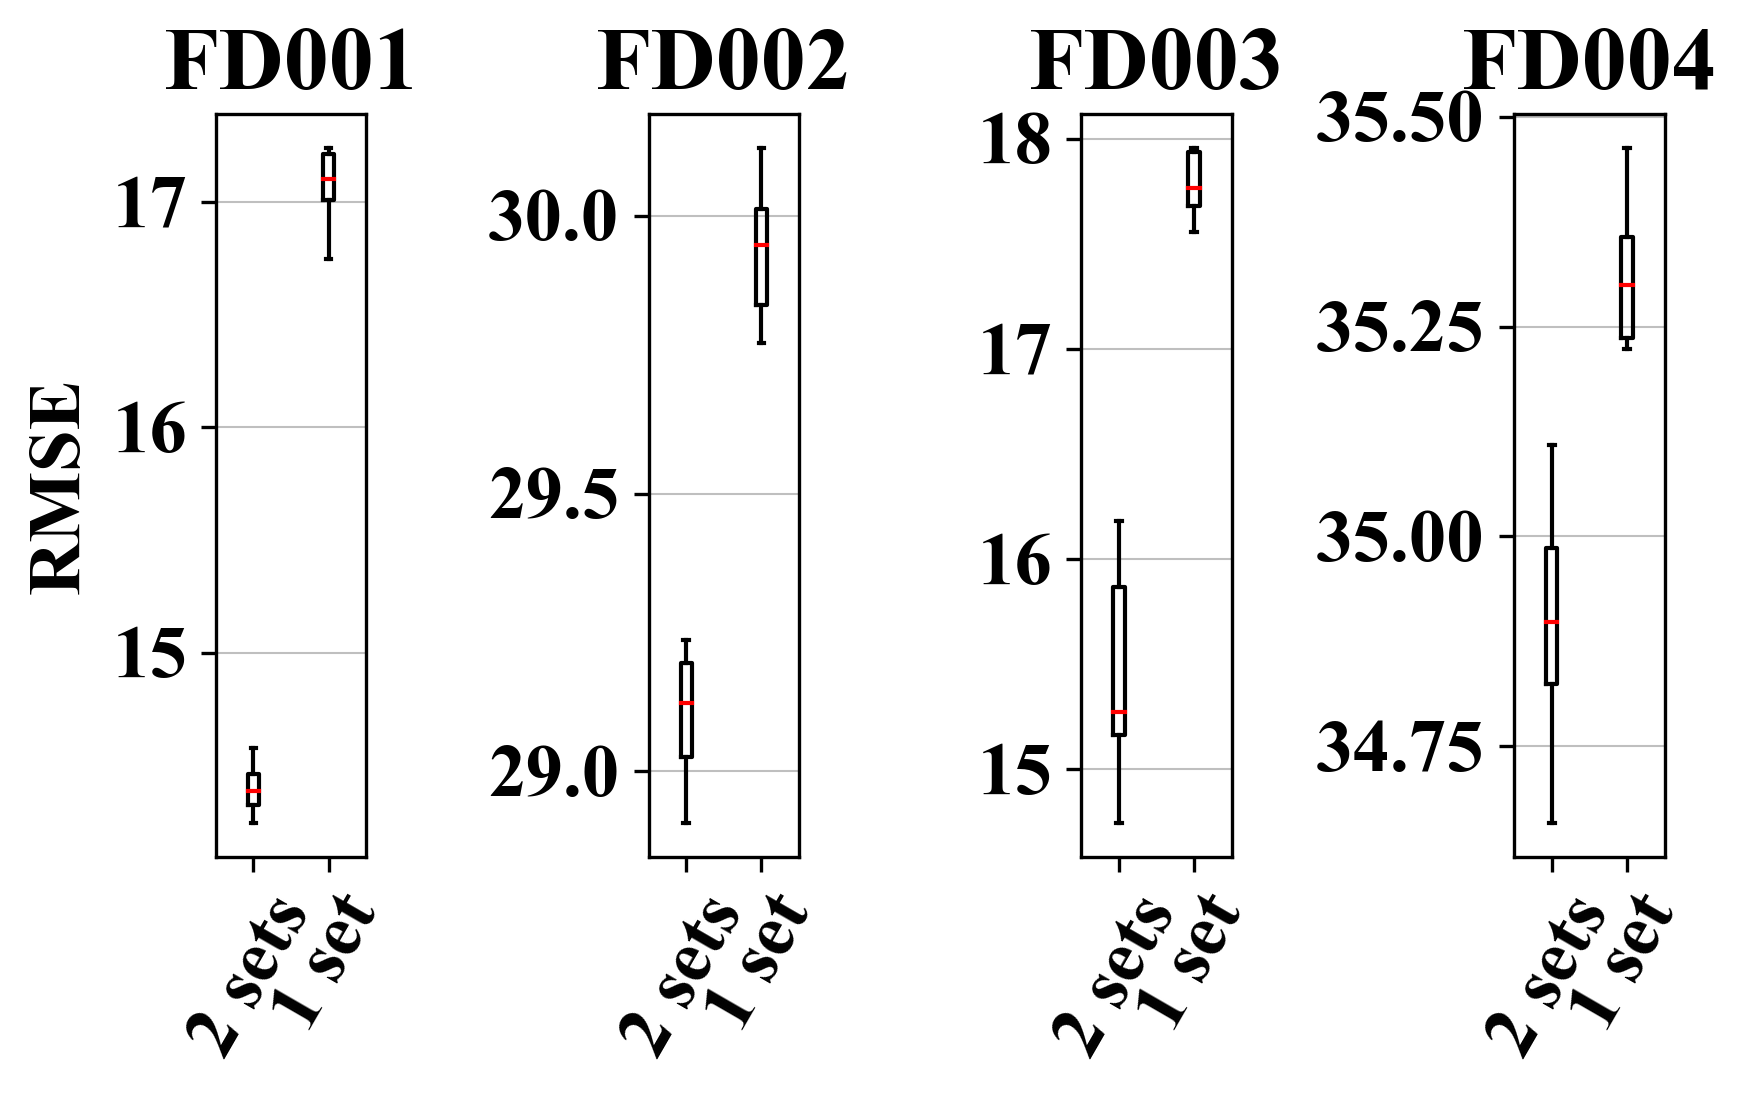
\includegraphics[width=0.5\textwidth]{img/rmse_comparisson.png}
\caption{Comparison of \gls{rmse} results for different sets of data-related parameters.}
\label{fig:scores_rmse}
\end{figure}

\begin{figure}[!htb]
\centering
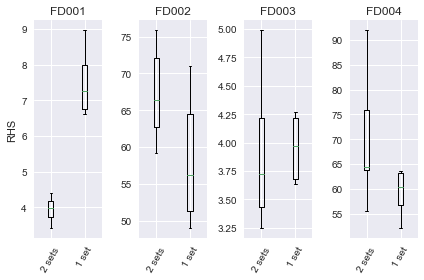
\includegraphics[width=0.5\textwidth]{img/rhs_comparisson.png}
\caption{Comparison of \gls{rhs} results for different sets of data-related parameters.}
\label{fig:scores_rhs}
\end{figure}
\section{Conclusions and future work}
\label{sec:conclusions}

This paper presents a novel framework for predicting the \gls{rul} of mechanical components. While the method was tested on the jet-engine specific dataset \gls{cmaps}, the method is general enough so that it can theoretically be applied to other kind of similar systems. The framework makes use of a strided moving time window to generate the training and test sets, a shallow \gls{mlp} to make the predictions of the \gls{rul} and an evolutionary algorithm (\gls{de}) which needs to be run just once in order to find the best data-related parameters that optimize the scoring functions used in this study.  The results presented in this paper demonstrate that the proposed framework is accurate and computationally efficient, which makes this framework suitable for applications that have limited computational resources such as embedded systems. Furthermore, a comparison with other state-of-the-art methods shown that the proposed method is the best overall performer. 

Two major features of the proposed framework are its generality and scalability. While for this paper very specific regressors and evolutionary algorithms were chosen, many other combinations are possible and may be more suitable for different applications. Furthermore, the framework here presented can, in principle, be used for model-construction, i.e. generating the best possible neural network architecture tailored to a specific application. Both issues are to be addressed in future work.
\pagebreak
\appendix
%\addcontentsline{toc}{section}{Appendices}
%\section*{Appendices}
\section{Tested Neural Network Architectures}
\label{sec:appendices}

Architecture 1

\begin{table}[!htb]
\centering
\begin{tabular}{l l l l}
	\hline
	Layer & Shape & Activation & Additional Information\\
  	\hline
  	Fully connected & 250 & ReLU & L1 = 0.1, L2 = 0.2\\
  	Fully connected & 50 & ReLU & L1 = 0.1, L2 = 0.2\\
  	Fully connected & 1 & Linear & L1 = 0.1, L2 = 0.2\\
  	\hline
\end{tabular}
\caption{Proposed Neural Network architecture 4}
\label{table:proposed_nn_4}
\end{table}

Architecture 2

\begin{table}[!htb]
\centering
\begin{tabular}{l l l l}
	\hline
	Layer & Shape & Activation & Additional Information\\
  	\hline
  	Fully connected & 100 & ReLU & L1 = 0.1, L2 = 0.2\\
  	Fully connected & 50 & ReLU & L1 = 0.1, L2 = 0.2\\
  	Fully connected & 1 & Linear & L1 = 0.1, L2 = 0.2\\
  	\hline
\end{tabular}
\caption{Proposed Neural Network architecture 3}
\label{table:proposed_nn_3}
\end{table}

Architecture 3

\begin{table}[!htb]
\centering
\begin{tabular}{l l l l}
	\hline
	Layer & Shape & Activation & Additional Information\\
  	\hline
  	Fully connected & 50 & ReLU & L1 = 0.1, L2 = 0.2\\
  	Fully connected & 20 & ReLU & L1 = 0.1, L2 = 0.2\\
  	Fully connected & 1 & Linear & L1 = 0.1, L2 = 0.2\\
  	\hline
\end{tabular}
\caption{Proposed Neural Network architecture 2}
\label{table:proposed_nn_2}
\end{table}

Architecture 4

\begin{table}[!htb]
\centering
\begin{tabular}{l l l l}
	\hline
	Layer & Shape & Activation & Additional Information\\
  	\hline
  	Fully connected & 20 & ReLU & L1 = 0.1, L2 = 0.2\\
  	Fully connected & 20 & ReLU & L1 = 0.1, L2 = 0.2\\
  	Fully connected & 1 & Linear & L1 = 0.1, L2 = 0.2\\
  	\hline
\end{tabular}
\caption{Proposed Neural Network architecture 1}
\label{table:proposed_nn_1}
\end{table}

Architecture 5

\begin{table}[!htb]
\centering
\begin{tabular}{l l l l}
	\hline
	Layer & Shape & Activation & Additional Information\\
  	\hline
  	Fully connected & 20 & ReLU & L1 = 0.1, L2 = 0.2\\
  	Fully connected & 1 & Linear & L1 = 0.1, L2 = 0.2\\
  	\hline
\end{tabular}
\caption{Proposed Neural Network architecture 5}
\label{table:proposed_nn_5}
\end{table}

\pagebreak

Architecture 6

\begin{table}[!htb]
\centering
\begin{tabular}{l l l l}
	\hline
	Layer & Shape & Activation & Additional Information\\
  	\hline
  	Fully connected & 10 & ReLU & L1 = 0.1, L2 = 0.2\\
  	Fully connected & 1 & Linear & L1 = 0.1, L2 = 0.2\\
  	\hline
\end{tabular}
\caption{Proposed Neural Network architecture 6}
\label{table:proposed_nn_6}
\end{table}

%------------------------------------------------


\vskip 0.2in
\bibliography{../reference_rul_paper}

\end{document}